\documentclass[10pt,a4paper,draft]{article}
\usepackage[utf8x]{inputenc}
\usepackage{ucs}
\usepackage[english]{babel}
\usepackage{multirow}
\usepackage{rotating}
\author{Lukáš Petrovický}
\title{RAS2012: Competition Entry}
\begin{document}

\maketitle

\begin{abstract}
This article describes an entry to the 2012 RAS Problem Solving Competition, concerning dispatching on multi-track territories. The entry is based on the Drools Planner, a Java-based solver. On a reasonably recent computer, the resulting algorithm is able to produce feasible results within a minute and has been fine-tuned to provide best results in under 3 minutes. Source code to the entry is open source and well documented.
\end{abstract}

\section{Introduction}

\section{Describing the solution}

\section{Implementation}

\section{Conclusion}

\appendix

\section{Resolved systems}

In this section, we show the best solutions reached for each data set. All these were reached within 3 minutes in a single-threaded run, using Intel i7 Q820 processor running Fedora 17 and 1 GB of heap space inside Java 7 runtime environment. The specific solver configurations used to reach these solutions may not have been the same every time.

Please note that via the benchmarking functionality of Drools planner (see above), users may be able to fine-tune the algorithm. This fine-tuning can be focused either on providing better solutions or on faster turnaround times.

\begin{sidewaystable}
\footnotesize
\caption{Statistics for resolved system ``RAS DATA SET 1'', costing \$1386.}
\centering
\begin{tabular}{c||c|c||c|c|c|c|c||c|c|c}
  \hline \hline
  &
  Unpref. & 
  Delay &
  Node &
  When &
  SA &
  +/- &
  Pty &
  TWT &
  +/- &
  Pty \\
      \hline
      \multirow{2}{*}{A1} &
      \multirow{2}{*}{0} &
      \multirow{2}{*}{0} &
      37 &
      2398.5 &
      3600 &
        1201.5 &
        0 &
      \multirow{2}{*}{5400} &
        \multirow{2}{*}{67.5} &
        \multirow{2}{*}{0}
      \\
      \cline{4-8}
       &
       &
       &
      39 &
      5332.5 &
      7800 &
        2467.5 &
        0 &
      
         &
        
      \\
      \hline
      \multirow{2}{*}{A2} &
      \multirow{2}{*}{0} &
      \multirow{2}{*}{0} &
      37 &
      6124.742 &
      7800 &
        1675.258 &
        0 &
      \multirow{2}{*}{9000} &
        \multirow{2}{*}{197.99} &
        \multirow{2}{*}{0}
      \\
      \cline{4-8}
       &
       &
       &
      39 &
      8802.01 &
      12000 &
        3197.99 &
        0 &
      
         &
        
      \\
      \hline
      \multirow{2}{*}{B1} &
      \multirow{2}{*}{11} &
      \multirow{2}{*}{3420} &
      37 &
      12886.282 &
      12600 &
        -286.282 &
        0 &
      \multirow{2}{*}{13800} &
        \multirow{2}{*}{-3835.319} &
        \multirow{2}{*}{0}
      \\
      \cline{4-8}
       &
       &
       &
      0 &
      17635.319 &
      17400 &
        -235.319 &
        0 &
      
         &
        
      \\
      \hline
      \multirow{2}{*}{B2} &
      \multirow{2}{*}{4} &
      \multirow{2}{*}{0} &
      37 &
      13621.758 &
      15600 &
        1978.242 &
        0 &
      \multirow{2}{*}{16800} &
        \multirow{2}{*}{82.248} &
        \multirow{2}{*}{0}
      \\
      \cline{4-8}
       &
       &
       &
      39 &
      16717.752 &
      19800 &
        3082.248 &
        0 &
      
         &
        
      \\
      \hline
      \multirow{2}{*}{B3} &
      \multirow{2}{*}{8} &
      \multirow{2}{*}{0} &
      37 &
      39096.616 &
      40200 &
        1103.384 &
        0 &
      \multirow{2}{*}{42000} &
        \multirow{2}{*}{-352.165} &
        \multirow{2}{*}{0}
      \\
      \cline{4-8}
       &
       &
       &
      39 &
      42352.165 &
      45000 &
        2647.835 &
        0 &
      
         &
        
      \\
      \hline
      \multirow{2}{*}{C1} &
      \multirow{2}{*}{0} &
      \multirow{2}{*}{0} &
      37 &
      17598 &
      19200 &
        1602 &
        0 &
      \multirow{2}{*}{21600} &
        \multirow{2}{*}{282} &
        \multirow{2}{*}{0}
      \\
      \cline{4-8}
       &
       &
       &
      39 &
      21318 &
      24600 &
        3282 &
        0 &
      
         &
        
      \\
      \hline
      \multirow{2}{*}{C2} &
      \multirow{2}{*}{0} &
      \multirow{2}{*}{240} &
      37 &
      25603.288 &
      27000 &
        1396.712 &
        0 &
      \multirow{2}{*}{28800} &
        \multirow{2}{*}{-747.861} &
        \multirow{2}{*}{0}
      \\
      \cline{4-8}
       &
       &
       &
      39 &
      29547.861 &
      33000 &
        3452.139 &
        0 &
      
         &
        
      \\
      \hline
      \multirow{2}{*}{D1} &
      \multirow{2}{*}{0} &
      \multirow{2}{*}{0} &
      37 &
      26334.852 &
      29400 &
        3065.148 &
        0 &
      \multirow{2}{*}{31200} &
        \multirow{2}{*}{296.584} &
        \multirow{2}{*}{0}
      \\
      \cline{4-8}
       &
       &
       &
      0 &
      30903.416 &
      36600 &
        5696.584 &
        0 &
      
         &
        
      \\
      \hline
      \multirow{2}{*}{D2} &
      \multirow{2}{*}{10} &
      \multirow{2}{*}{2400} &
      37 &
      21320.177 &
      21600 &
        279.823 &
        0 &
      \multirow{2}{*}{23400} &
        \multirow{2}{*}{-2345.604} &
        \multirow{2}{*}{0}
      \\
      \cline{4-8}
       &
       &
       &
      0 &
      25745.604 &
      28200 &
        2454.396 &
        0 &
      
         &
        
      \\
      \hline
      \multirow{2}{*}{D3} &
      \multirow{2}{*}{0} &
      \multirow{2}{*}{5520} &
      37 &
      38388.738 &
      35400 &
        -2988.738 &
        0 &
      \multirow{2}{*}{37200} &
        \multirow{2}{*}{-5327.639} &
        \multirow{2}{*}{0}
      \\
      \cline{4-8}
       &
       &
       &
      0 &
      42527.639 &
      41400 &
        -1127.639 &
        0 &
      
         &
        
      \\
      \hline
      \multirow{2}{*}{E1} &
      \multirow{2}{*}{26} &
      \multirow{2}{*}{3060} &
      37 &
      36597 &
      36000 &
        -597 &
        0 &
      \multirow{2}{*}{39000} &
        \multirow{2}{*}{-2625} &
        \multirow{2}{*}{0}
      \\
      \cline{4-8}
       &
       &
       &
      39 &
      41625 &
      44400 &
        2775 &
        0 &
      
         &
        
      \\
      \hline
      \multirow{2}{*}{F1} &
      \multirow{2}{*}{0} &
      \multirow{2}{*}{1440} &
      37 &
      52205.142 &
      57600 &
        \multicolumn{2}{|c||}{N/A} &
      \multirow{2}{*}{63000} &
        \multicolumn{2}{c}{\multirow{2}{*}{N/A}}
      \\
      \cline{4-8}
       &
       &
       &
      0 &
      63197.997 &
      75000 &
        \multicolumn{2}{|c||}{N/A} &
      
        
      \\
\end{tabular}
\label{table:RDS1.txt-1386.tex} 
\end{sidewaystable}.

\begin{sidewaystable}
\footnotesize
\caption{Statistics for resolved system ``RAS DATA SET 2'', costing \$7337.}
\centering
\begin{tabular}{c||c|c||c|c|c|c|c||c|c|c}
  \hline \hline
  &
  Unpref. & 
  Delay &
  Node &
  When &
  SA &
  +/- &
  Pty &
  TWT &
  +/- &
  Pty \\
      \hline
      \multirow{2}{*}{A1} &
      \multirow{2}{*}{0} &
      \multirow{2}{*}{60} &
      37 &
      3142.5 &
      3600 &
        457.5 &
        0 &
      \multirow{2}{*}{5400} &
        \multirow{2}{*}{-1063.5} &
        \multirow{2}{*}{0}
      \\
      \cline{4-8}
       &
       &
       &
      39 &
      6463.5 &
      7800 &
        1336.5 &
        0 &
      
         &
        
      \\
      \hline
      \multirow{2}{*}{A2} &
      \multirow{2}{*}{8} &
      \multirow{2}{*}{720} &
      37 &
      11146.424 &
      11400 &
        253.576 &
        0 &
      \multirow{2}{*}{12600} &
        \multirow{2}{*}{-1664.533} &
        \multirow{2}{*}{0}
      \\
      \cline{4-8}
       &
       &
       &
      39 &
      14264.533 &
      15600 &
        1335.467 &
        0 &
      
         &
        
      \\
      \hline
      \multirow{2}{*}{A3} &
      \multirow{2}{*}{4} &
      \multirow{2}{*}{0} &
      37 &
      17185.5 &
      18000 &
        814.5 &
        0 &
      \multirow{2}{*}{19800} &
        \multirow{2}{*}{-49.5} &
        \multirow{2}{*}{0}
      \\
      \cline{4-8}
       &
       &
       &
      39 &
      19849.5 &
      22200 &
        2350.5 &
        0 &
      
         &
        
      \\
      \hline
      \multirow{2}{*}{A4} &
      \multirow{2}{*}{26} &
      \multirow{2}{*}{60} &
      37 &
      36235.943 &
      31800 &
        -4435.943 &
        0 &
      \multirow{2}{*}{39000} &
        \multirow{2}{*}{-757.857} &
        \multirow{2}{*}{0}
      \\
      \cline{4-8}
       &
       &
       &
      0 &
      39757.857 &
      36600 &
        -3157.857 &
        0 &
      
         &
        
      \\
      \hline
      \multirow{2}{*}{B1} &
      \multirow{2}{*}{9} &
      \multirow{2}{*}{0} &
      37 &
      7064.466 &
      4800 &
        -2264.466 &
        0 &
      \multirow{2}{*}{9600} &
        \multirow{2}{*}{-814.578} &
        \multirow{2}{*}{0}
      \\
      \cline{4-8}
       &
       &
       &
      39 &
      10414.578 &
      9000 &
        -1414.578 &
        0 &
      
         &
        
      \\
      \hline
      \multirow{2}{*}{B2} &
      \multirow{2}{*}{20} &
      \multirow{2}{*}{1020} &
      37 &
      33175.875 &
      26400 &
        -6775.875 &
        0 &
      \multirow{2}{*}{35400} &
        \multirow{2}{*}{-907.875} &
        \multirow{2}{*}{0}
      \\
      \cline{4-8}
       &
       &
       &
      39 &
      36307.875 &
      31200 &
        -5107.875 &
        0 &
      
         &
        
      \\
      \hline
      \multirow{2}{*}{B3} &
      \multirow{2}{*}{0} &
      \multirow{2}{*}{15357.855} &
      37 &
      22527 &
      11400 &
        -11127 &
        218 &
      \multirow{2}{*}{10800} &
        \multirow{2}{*}{-15153.431} &
        \multirow{2}{*}{90}
      \\
      \cline{4-8}
       &
       &
       &
      0 &
      25953.431 &
      16800 &
        -9153.431 &
        108 &
      
         &
        
      \\
      \hline
      \multirow{2}{*}{C1} &
      \multirow{2}{*}{11} &
      \multirow{2}{*}{0} &
      37 &
      35829.006 &
      26400 &
        -9429.006 &
        123 &
      \multirow{2}{*}{39000} &
        \multirow{2}{*}{-148.856} &
        \multirow{2}{*}{0}
      \\
      \cline{4-8}
       &
       &
       &
      39 &
      39148.856 &
      31800 &
        -7348.856 &
        8 &
      
         &
        
      \\
      \hline
      \multirow{2}{*}{C2} &
      \multirow{2}{*}{0} &
      \multirow{2}{*}{1260} &
      37 &
      198 &
      0 &
        -198 &
        0 &
      \multirow{2}{*}{3600} &
        \multirow{2}{*}{-1578} &
        \multirow{2}{*}{0}
      \\
      \cline{4-8}
       &
       &
       &
      39 &
      5178 &
      5400 &
        222 &
        0 &
      
         &
        
      \\
      \hline
      \multirow{2}{*}{C3} &
      \multirow{2}{*}{19} &
      \multirow{2}{*}{1920} &
      37 &
      23633.144 &
      20400 &
        -3233.144 &
        0 &
      \multirow{2}{*}{25200} &
        \multirow{2}{*}{-2196.432} &
        \multirow{2}{*}{0}
      \\
      \cline{4-8}
       &
       &
       &
      0 &
      27396.432 &
      25800 &
        -1596.432 &
        0 &
      
         &
        
      \\
      \hline
      \multirow{2}{*}{D1} &
      \multirow{2}{*}{0} &
      \multirow{2}{*}{0} &
      37 &
      40615.5 &
      43800 &
        3184.5 &
        0 &
      \multirow{2}{*}{44400} &
        \multicolumn{2}{c}{\multirow{2}{*}{N/A}}
      \\
      \cline{4-8}
       &
       &
       &
      39 &
      44812.5 &
      51000 &
        \multicolumn{2}{|c||}{N/A} &
      
        
      \\
      \hline
      \multirow{2}{*}{D2} &
      \multirow{2}{*}{0} &
      \multirow{2}{*}{0} &
      37 &
      1855.382 &
      3600 &
        1744.618 &
        0 &
      \multirow{2}{*}{6600} &
        \multirow{2}{*}{864.932} &
        \multirow{2}{*}{0}
      \\
      \cline{4-8}
       &
       &
       &
      39 &
      5735.068 &
      9600 &
        3864.932 &
        0 &
      
         &
        
      \\
      \hline
      \multirow{2}{*}{E1} &
      \multirow{2}{*}{0} &
      \multirow{2}{*}{54600} &
      37 &
      59453.456 &
      6600 &
        \multicolumn{2}{|c||}{N/A} &
      \multirow{2}{*}{9600} &
        \multicolumn{2}{c}{\multirow{2}{*}{N/A}}
      \\
      \cline{4-8}
       &
       &
       &
      39 &
      63976.367 &
      14400 &
        \multicolumn{2}{|c||}{N/A} &
      
        
      \\
      \hline
      \multirow{2}{*}{E2} &
      \multirow{2}{*}{0} &
      \multirow{2}{*}{1020} &
      37 &
      2154.858 &
      1800 &
        -354.858 &
        0 &
      \multirow{2}{*}{7200} &
        \multirow{2}{*}{-1046.294} &
        \multirow{2}{*}{0}
      \\
      \cline{4-8}
       &
       &
       &
      0 &
      8246.294 &
      10800 &
        2553.706 &
        0 &
      
         &
        
      \\
      \hline
      \multirow{2}{*}{E3} &
      \multirow{2}{*}{13} &
      \multirow{2}{*}{60} &
      37 &
      6107.998 &
      9000 &
        2892.002 &
        0 &
      \multirow{2}{*}{12000} &
        \multirow{2}{*}{26.575} &
        \multirow{2}{*}{0}
      \\
      \cline{4-8}
       &
       &
       &
      0 &
      11973.425 &
      18000 &
        6026.575 &
        0 &
      
         &
        
      \\
      \hline
      \multirow{2}{*}{E4} &
      \multirow{2}{*}{15} &
      \multirow{2}{*}{0} &
      37 &
      27424.521 &
      30000 &
        2575.479 &
        0 &
      \multirow{2}{*}{32400} &
        \multirow{2}{*}{-179.3} &
        \multirow{2}{*}{0}
      \\
      \cline{4-8}
       &
       &
       &
      0 &
      32579.3 &
      37800 &
        5220.7 &
        0 &
      
         &
        
      \\
      \hline
      \multirow{2}{*}{F1} &
      \multirow{2}{*}{0} &
      \multirow{2}{*}{22200} &
      37 &
      47408.18 &
      29400 &
        \multicolumn{2}{|c||}{N/A} &
      \multirow{2}{*}{33600} &
        \multicolumn{2}{c}{\multirow{2}{*}{N/A}}
      \\
      \cline{4-8}
       &
       &
       &
      39 &
      54958.362 &
      41400 &
        \multicolumn{2}{|c||}{N/A} &
      
        
      \\
      \hline
      \multirow{2}{*}{F2} &
      \multirow{2}{*}{0} &
      \multirow{2}{*}{34680} &
      37 &
      55870.288 &
      30000 &
        \multicolumn{2}{|c||}{N/A} &
      \multirow{2}{*}{36000} &
        \multicolumn{2}{c}{\multirow{2}{*}{N/A}}
      \\
      \cline{4-8}
       &
       &
       &
      0 &
      69216.861 &
      51000 &
        \multicolumn{2}{|c||}{N/A} &
      
        
      \\
\end{tabular}
\label{table:RDS2.txt-7337.tex} 
\end{sidewaystable}.

\begin{sidewaystable}
\footnotesize
\caption{Statistics for resolved system ``RAS DATA SET 3'', costing \$10563.}
\centering
\begin{tabular}{c||c|c||c|c|c|c|c||c|c|c}
  \hline \hline
  &
  Unpref. & 
  Delay &
  Node &
  When &
  SA &
  +/- &
  Pty &
  TWT &
  +/- &
  Pty \\
      \hline
      \multirow{2}{*}{A1} &
      \multirow{2}{*}{0} &
      \multirow{2}{*}{0} &
      37 &
      967.5 &
      2400 &
        1432.5 &
        0 &
      \multirow{2}{*}{4200} &
        \multirow{2}{*}{685.5} &
        \multirow{2}{*}{0}
      \\
      \cline{4-8}
       &
       &
       &
      39 &
      3514.5 &
      6000 &
        2485.5 &
        0 &
      
         &
        
      \\
      \hline
      \multirow{2}{*}{A2} &
      \multirow{2}{*}{23} &
      \multirow{2}{*}{3840} &
      37 &
      2280 &
      2400 &
        120 &
        0 &
      \multirow{2}{*}{4200} &
        \multirow{2}{*}{-4842.003} &
        \multirow{2}{*}{0}
      \\
      \cline{4-8}
       &
       &
       &
      0 &
      9042.003 &
      6600 &
        -2442.003 &
        0 &
      
         &
        
      \\
      \hline
      \multirow{2}{*}{A3} &
      \multirow{2}{*}{24} &
      \multirow{2}{*}{240} &
      37 &
      21881.146 &
      22800 &
        918.854 &
        0 &
      \multirow{2}{*}{24000} &
        \multirow{2}{*}{-902.579} &
        \multirow{2}{*}{0}
      \\
      \cline{4-8}
       &
       &
       &
      0 &
      24902.579 &
      27000 &
        2097.421 &
        0 &
      
         &
        
      \\
      \hline
      \multirow{2}{*}{A4} &
      \multirow{2}{*}{15} &
      \multirow{2}{*}{7500} &
      37 &
      43787.461 &
      33600 &
        \multicolumn{2}{|c||}{N/A} &
      \multirow{2}{*}{39000} &
        \multicolumn{2}{c}{\multirow{2}{*}{N/A}}
      \\
      \cline{4-8}
       &
       &
       &
      0 &
      47399.375 &
      38400 &
        \multicolumn{2}{|c||}{N/A} &
      
        
      \\
      \hline
      \multirow{2}{*}{A5} &
      \multirow{2}{*}{0} &
      \multirow{2}{*}{4815} &
      37 &
      36697.5 &
      32400 &
        -4297.5 &
        0 &
      \multirow{2}{*}{34200} &
        \multirow{2}{*}{-5044.5} &
        \multirow{2}{*}{0}
      \\
      \cline{4-8}
       &
       &
       &
      39 &
      39244.5 &
      36600 &
        -2644.5 &
        0 &
      
         &
        
      \\
      \hline
      \multirow{1}{*}{B1} &
      \multirow{1}{*}{0} &
      \multirow{1}{*}{4680} &
      0 &
      6166.284 &
      1800 &
        -4366.284 &
        0 &
      \multirow{1}{*}{1200} &
        \multirow{1}{*}{-4966.284} &
        \multirow{1}{*}{0}
      \\
      \hline
      \multirow{1}{*}{B2} &
      \multirow{1}{*}{0} &
      \multirow{1}{*}{0} &
      39 &
      2869.163 &
      4800 &
        1930.837 &
        0 &
      \multirow{1}{*}{3000} &
        \multirow{1}{*}{130.837} &
        \multirow{1}{*}{0}
      \\
      \hline
      \multirow{2}{*}{B3} &
      \multirow{2}{*}{14} &
      \multirow{2}{*}{3180} &
      37 &
      5694.95 &
      -3000 &
        -8694.95 &
        83 &
      \multirow{2}{*}{6000} &
        \multirow{2}{*}{-2697.514} &
        \multirow{2}{*}{0}
      \\
      \cline{4-8}
       &
       &
       &
      39 &
      8697.514 &
      1800 &
        -6897.514 &
        0 &
      
         &
        
      \\
      \hline
      \multirow{2}{*}{B4} &
      \multirow{2}{*}{0} &
      \multirow{2}{*}{17700} &
      37 &
      46613.144 &
      16800 &
        \multicolumn{2}{|c||}{N/A} &
      \multirow{2}{*}{32400} &
        \multicolumn{2}{c}{\multirow{2}{*}{N/A}}
      \\
      \cline{4-8}
       &
       &
       &
      0 &
      50039.575 &
      21600 &
        \multicolumn{2}{|c||}{N/A} &
      
        
      \\
      \hline
      \multirow{1}{*}{C1} &
      \multirow{1}{*}{0} &
      \multirow{1}{*}{7260} &
      0 &
      10602.853 &
      6000 &
        -4602.853 &
        0 &
      \multirow{1}{*}{4200} &
        \multirow{1}{*}{-6402.853} &
        \multirow{1}{*}{0}
      \\
      \hline
      \multirow{2}{*}{C2} &
      \multirow{2}{*}{0} &
      \multirow{2}{*}{0} &
      37 &
      3426.431 &
      0 &
        -3426.431 &
        0 &
      \multirow{2}{*}{7200} &
        \multirow{2}{*}{-171.004} &
        \multirow{2}{*}{0}
      \\
      \cline{4-8}
       &
       &
       &
      39 &
      7371.004 &
      6000 &
        -1371.004 &
        0 &
      
         &
        
      \\
      \hline
      \multirow{2}{*}{C3} &
      \multirow{2}{*}{14} &
      \multirow{2}{*}{5880} &
      37 &
      33698.696 &
      30000 &
        -3698.696 &
        0 &
      \multirow{2}{*}{37200} &
        \multicolumn{2}{c}{\multirow{2}{*}{N/A}}
      \\
      \cline{4-8}
       &
       &
       &
      0 &
      43970.576 &
      36000 &
        \multicolumn{2}{|c||}{N/A} &
      
        
      \\
      \hline
      \multirow{2}{*}{D1} &
      \multirow{2}{*}{0} &
      \multirow{2}{*}{240} &
      37 &
      4253.996 &
      4200 &
        -53.996 &
        0 &
      \multirow{2}{*}{7800} &
        \multirow{2}{*}{-333.682} &
        \multirow{2}{*}{0}
      \\
      \cline{4-8}
       &
       &
       &
      39 &
      8133.682 &
      10200 &
        2066.318 &
        0 &
      
         &
        
      \\
      \hline
      \multirow{2}{*}{D2} &
      \multirow{2}{*}{20} &
      \multirow{2}{*}{0} &
      37 &
      39689.995 &
      42000 &
        2310.005 &
        0 &
      \multirow{2}{*}{43800} &
        \multicolumn{2}{c}{\multirow{2}{*}{N/A}}
      \\
      \cline{4-8}
       &
       &
       &
      39 &
      43852.145 &
      48000 &
        \multicolumn{2}{|c||}{N/A} &
      
        
      \\
      \hline
      \multirow{2}{*}{E1} &
      \multirow{2}{*}{45} &
      \multirow{2}{*}{11460} &
      37 &
      18231.433 &
      10200 &
        -8031.433 &
        0 &
      \multirow{2}{*}{13200} &
        \multirow{2}{*}{-11446.581} &
        \multirow{2}{*}{13}
      \\
      \cline{4-8}
       &
       &
       &
      0 &
      24646.581 &
      19200 &
        -5446.581 &
        0 &
      
         &
        
      \\
      \hline
      \multirow{2}{*}{E2} &
      \multirow{2}{*}{72} &
      \multirow{2}{*}{4374} &
      37 &
      17817 &
      18000 &
        183 &
        0 &
      \multirow{2}{*}{21000} &
        \multirow{2}{*}{-4659} &
        \multirow{2}{*}{0}
      \\
      \cline{4-8}
       &
       &
       &
      39 &
      25659 &
      26400 &
        741 &
        0 &
      
         &
        
      \\
      \hline
      \multirow{2}{*}{E3} &
      \multirow{2}{*}{14} &
      \multirow{2}{*}{0} &
      37 &
      19052.184 &
      21000 &
        1947.816 &
        0 &
      \multirow{2}{*}{24000} &
        \multirow{2}{*}{375.814} &
        \multirow{2}{*}{0}
      \\
      \cline{4-8}
       &
       &
       &
      39 &
      23624.186 &
      28800 &
        5175.814 &
        0 &
      
         &
        
      \\
      \hline
      \multirow{2}{*}{E4} &
      \multirow{2}{*}{0} &
      \multirow{2}{*}{2760} &
      37 &
      38308 &
      40800 &
        2492 &
        0 &
      \multirow{2}{*}{43800} &
        \multicolumn{2}{c}{\multirow{2}{*}{N/A}}
      \\
      \cline{4-8}
       &
       &
       &
      39 &
      46948 &
      49800 &
        \multicolumn{2}{|c||}{N/A} &
      
        
      \\
      \hline
      \multirow{2}{*}{F1} &
      \multirow{2}{*}{0} &
      \multirow{2}{*}{43200} &
      37 &
      54462.855 &
      18000 &
        \multicolumn{2}{|c||}{N/A} &
      \multirow{2}{*}{23400} &
        \multicolumn{2}{c}{\multirow{2}{*}{N/A}}
      \\
      \cline{4-8}
       &
       &
       &
      0 &
      65427.424 &
      34800 &
        \multicolumn{2}{|c||}{N/A} &
      
        
      \\
      \hline
      \multirow{2}{*}{F2} &
      \multirow{2}{*}{0} &
      \multirow{2}{*}{17760} &
      37 &
      51033 &
      37200 &
        \multicolumn{2}{|c||}{N/A} &
      \multirow{2}{*}{42000} &
        \multicolumn{2}{c}{\multirow{2}{*}{N/A}}
      \\
      \cline{4-8}
       &
       &
       &
      39 &
      59529 &
      51000 &
        \multicolumn{2}{|c||}{N/A} &
      
        
      \\
\end{tabular}
\label{table:RDS3.txt-10563.tex} 
\end{sidewaystable}.

\begin{sidewaystable}
\footnotesize
\caption{Statistics for resolved system ``RAS DATA SET TOY'', costing \$808.}
\centering
\begin{tabular}{c||c|c||c|c|c|c|c||c|c|c}
  \hline \hline
  &
  Unpref. & 
  Delay &
  Node &
  When &
  SA &
  +/- &
  Pty &
  TWT &
  +/- &
  Pty \\
      \hline
      \multirow{2}{*}{A1} &
      \multirow{2}{*}{0} &
      \multirow{2}{*}{1260} &
      6 &
      4260 &
      2400 &
        -1860 &
        0 &
      \multirow{2}{*}{8700} &
        \multirow{2}{*}{2640} &
        \multirow{2}{*}{0}
      \\
      \cline{4-8}
       &
       &
       &
      12 &
      6060 &
      4800 &
        -1260 &
        0 &
      
         &
        
      \\
      \hline
      \multirow{2}{*}{B1} &
      \multirow{2}{*}{0} &
      \multirow{2}{*}{3480} &
      6 &
      6283.16 &
      -3000 &
        -9283.16 &
        115 &
      \multirow{2}{*}{4800} &
        \multirow{2}{*}{-3903.328} &
        \multirow{2}{*}{0}
      \\
      \cline{4-8}
       &
       &
       &
      0 &
      8703.328 &
      5400 &
        -3303.328 &
        0 &
      
         &
        
      \\
      \hline
      \multirow{2}{*}{C1} &
      \multirow{2}{*}{0} &
      \multirow{2}{*}{0} &
      6 &
      2400 &
      3000 &
        600 &
        0 &
      \multirow{2}{*}{7200} &
        \multirow{2}{*}{2400} &
        \multirow{2}{*}{0}
      \\
      \cline{4-8}
       &
       &
       &
      12 &
      4800 &
      6000 &
        1200 &
        0 &
      
         &
        
      \\
\end{tabular}
\label{table:TOY.txt-808.tex} 
\end{sidewaystable}.

\section{Visualizations}

\begin{figure}
\centering
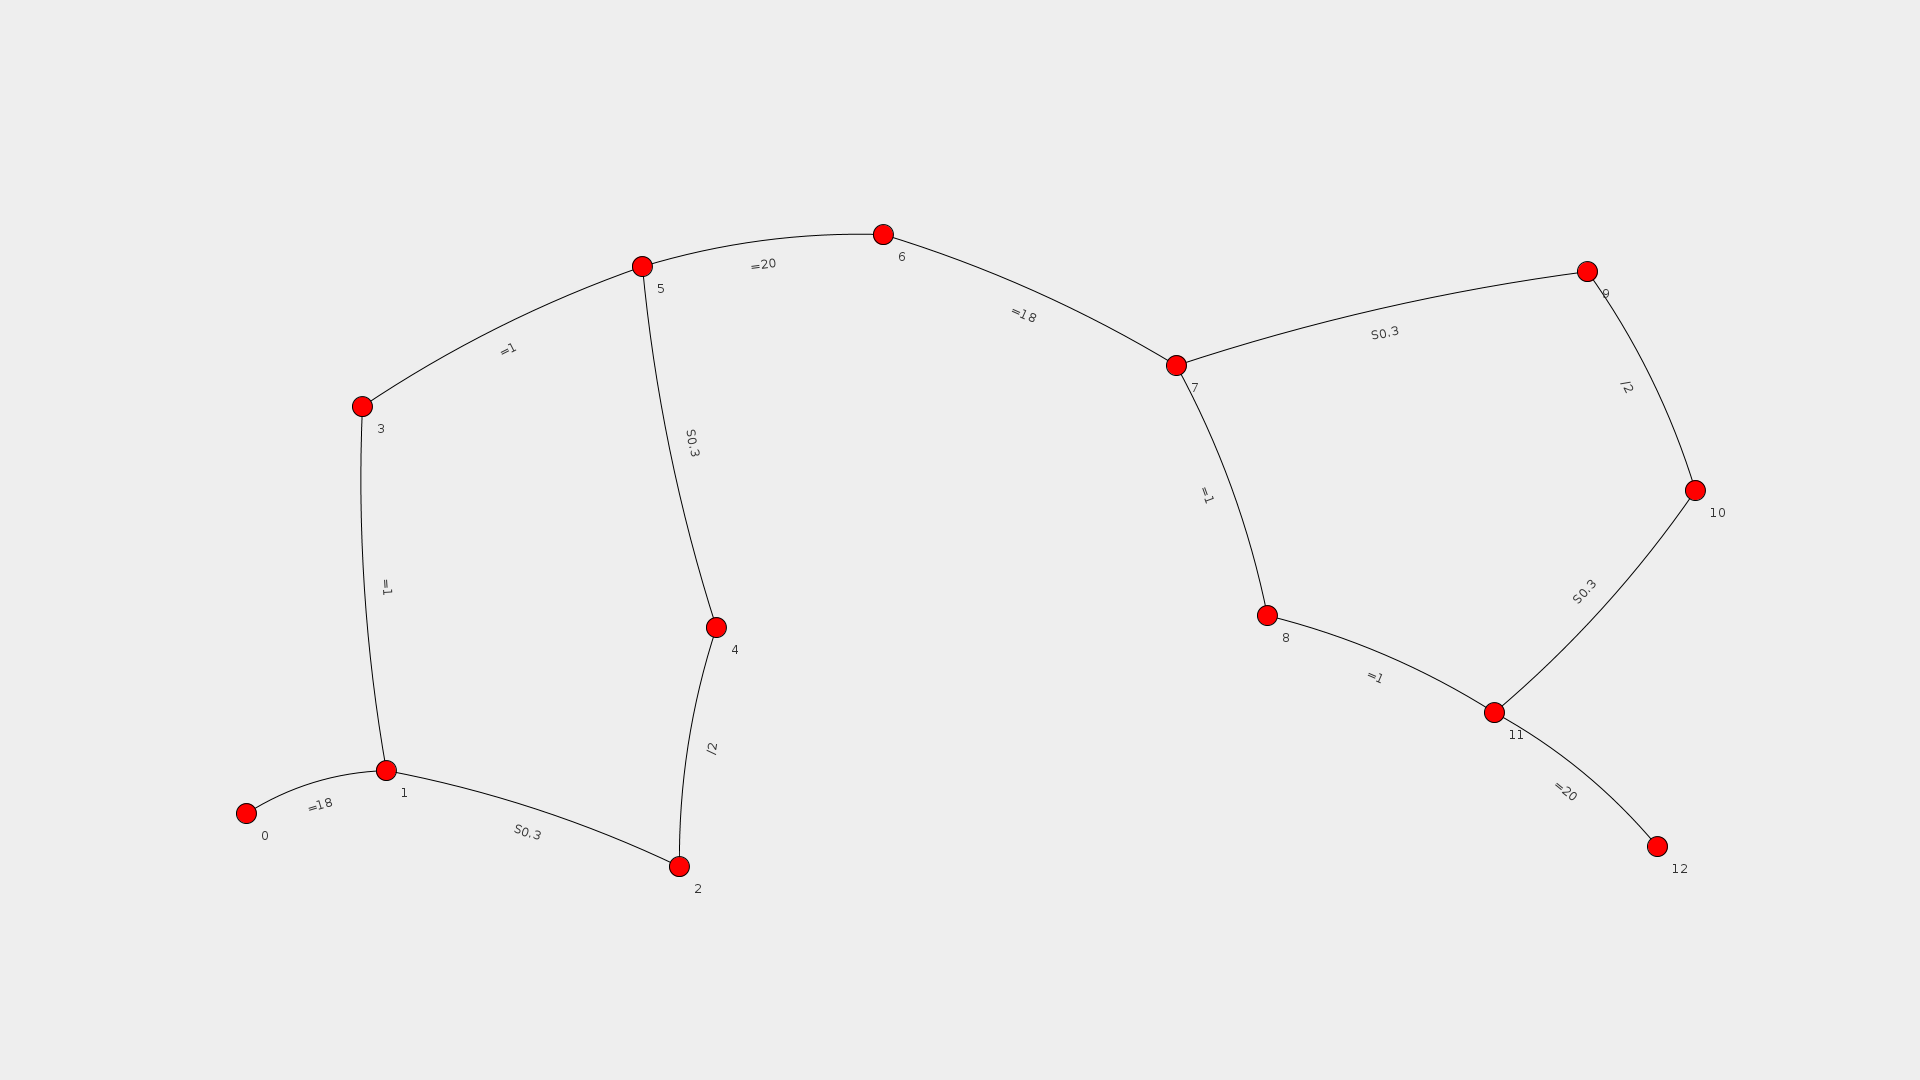
\includegraphics[width=150mm,angle=90]{solution.png}
\caption{RAS DATA SET TOY example territory. Undirected graph, arcs have descriptions.}
\end{figure}

\begin{figure}
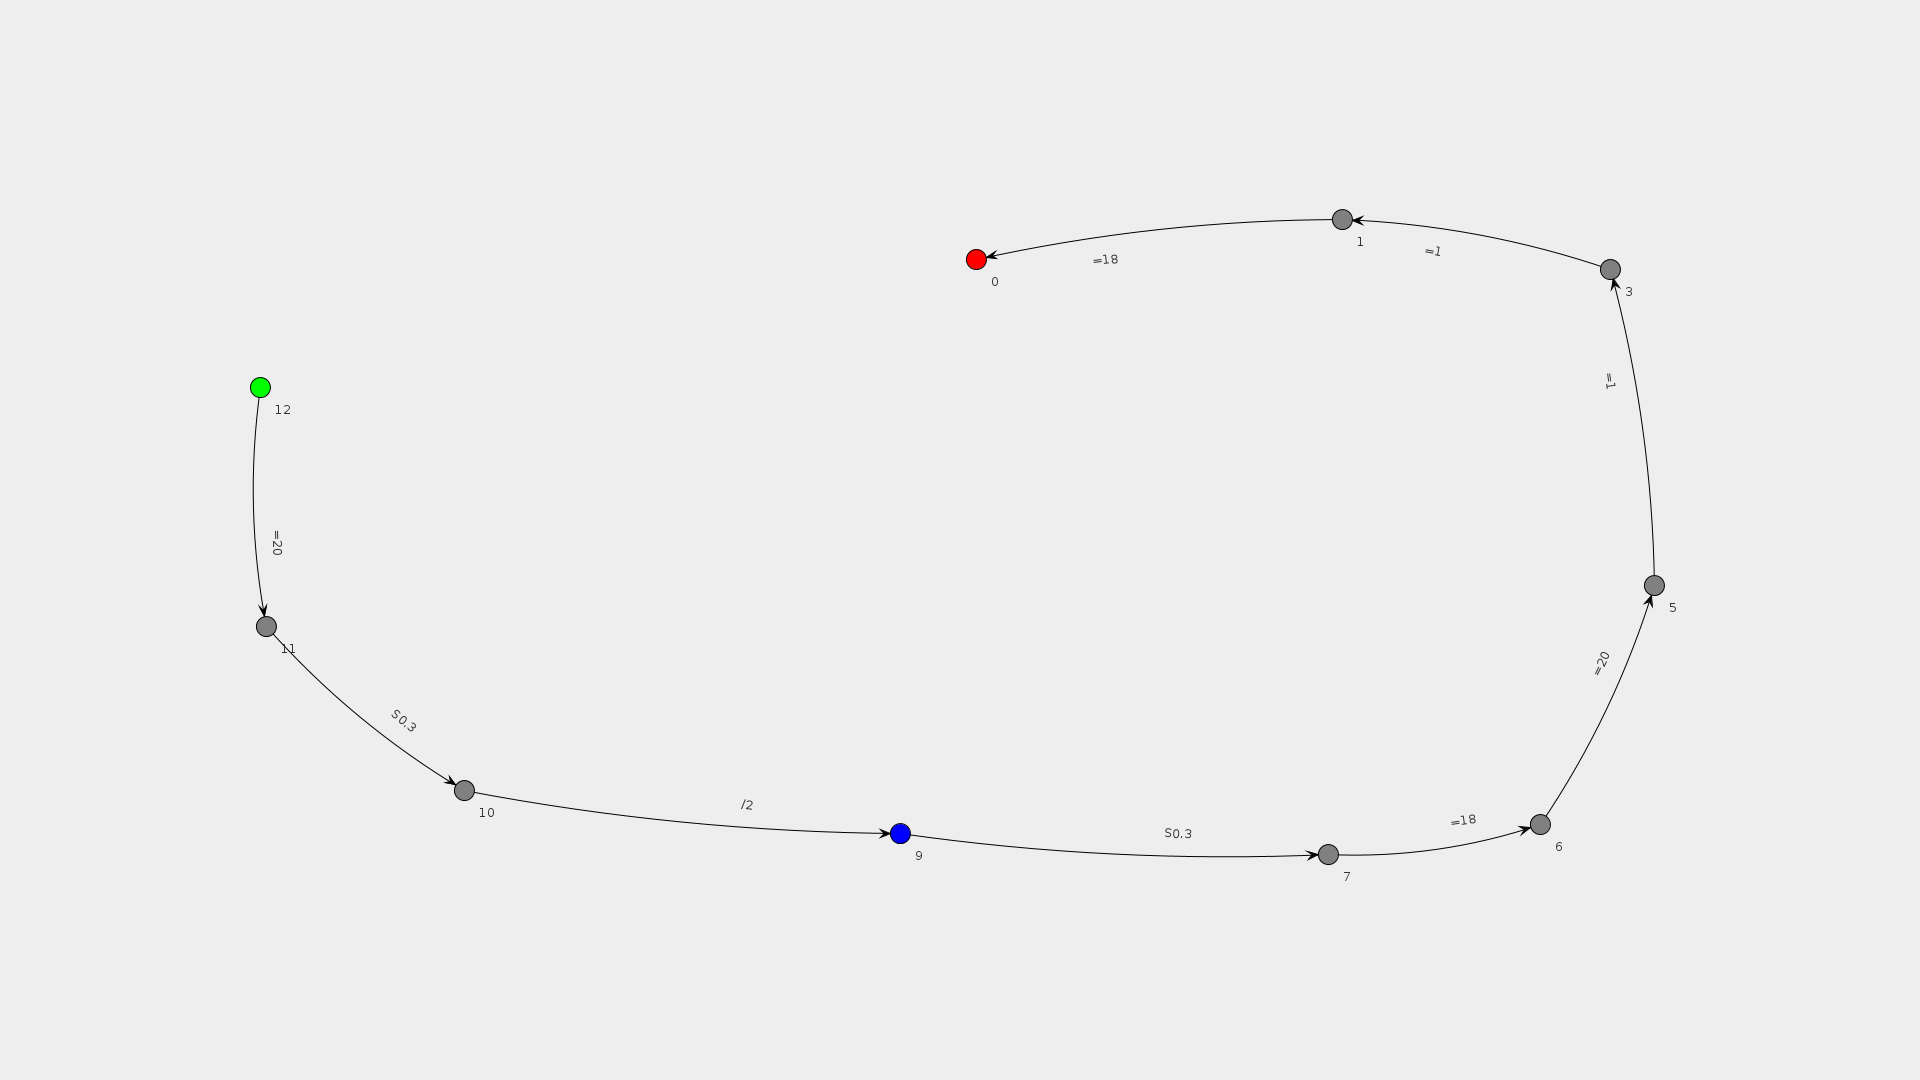
\includegraphics[width=150mm,angle=90]{B1.png}
\centering
\caption{RAS DATA SET TOY example, route of Train B1. Directed graph where green marks the origin, red the destination and blue is where the train is allowed to wait.}
\end{figure}

In this section, we show examples of visualizations that the solution is capable of providing. These visualizations have been rendered on the fly using the JUNG library\footnote{Java Universal Network/Graph framework, http://jung.sourceforge.net}.

\end{document}
